\chapter{Operating and Fault Scenarios}
\label{chap:scenarios}
% Traceability: ADR-001 ADR-002 ADR-003 ADR-004 ADR-005 ADR-006

The previous chapters explained the architecture one topic at a time. This chapter follows complete operating stories across power, safety, state, timing, communication, and data.

Each scenario illustrates the architecture under a particular operating condition. All recoverable faults use the common recovery process at the end of this chapter.

Each scenario asks the same questions: What was the initial condition? What changed? How was it detected? What happened in hardware? What state followed? What evidence remained? What is required before operation can resume?

\section{Normal Startup, Acquisition, and Disarm}

The controller begins unpowered and unarmed. When external power is applied, the central eFuse qualifies the input and supplies protected \texttt{+12V}. The backplane utility converters start, and their rail-health outputs keep the shared system from becoming armable until the common rails are valid.

Each active board starts from safe defaults. Its detector protection relays remain open. The board establishes identity, communication, monitoring, local interlock power, and its state logic. It then checks the timing, power, shared health, and local conditions that apply to its role.

The host connects directly to the active boards and verifies each identity against the instrument inventory. It sends operational settings and loads required sequencer payloads while the system is in \texttt{IDLE}. Boards report Ready only when their applicable configuration and live conditions are valid.

Before arming, the host verifies that configuration and readiness match the intended operation. The host then asks main to arm. Main raises \texttt{EN}; each function board performs its own acceptance checks and completes \texttt{RUN.init}. After the arm-to-first-trigger guard, main may send acquisition \texttt{SYNC}. Function boards perform their local timing work, and video boards send science data directly to the host.

For a normal stop, main sends the falling \texttt{SYNC} event and boards complete their controlled acquisition stop. The controller may remain armed for another acquisition. When the host requests disarm, main drops \texttt{EN}. Hardware relay permission disappears before any remaining firmware cleanup. Boards return to safe \texttt{IDLE}.

While disarmed, host disconnection alone does not assert \texttt{OK}; hardware protection remains active. If another host connects, it may use retained settings and sequences after verifying that configuration and readiness match the intended operation. Changing hosts does not itself require a reload or an interlock trip.

Figure~\ref{fig:operating-sequence} shows the normal sequence.

\section{Arm Attempted While One Board Is Not Ready}

Assume the controller is safely in \texttt{IDLE}, but one required sequencer board has not completed its loading transaction. The board is Not Ready. It has not detected a hardware fault, so it does not pull \texttt{OK} low merely because configuration is incomplete.

The host should see the readiness status and avoid the arm request. If an arm is attempted anyway, main may know only its own readiness and the shared health state. It raises \texttt{EN} only if its local checks pass.

The Not Ready function board then performs its independent arm acceptance. Because a required condition is missing, it does not request local relay permission. An unsafe arm attempt uses the board's normal trip path, pulling \texttt{OK} low and placing the fleet in the safe error state.

Diagnostics show that the initiating board rejected the arm because it was not ready. The host clears the error through the normal recovery path, loads the missing sequencer, verifies readiness, and arms again. There is no separate shared readiness wire and no way for the host to force the local board to accept the arm.

\section{Three Different Power-Loss Cases}

Power faults can look similar to an operator because detector-facing outputs turn off in every case. Their detection and remaining diagnostic capability differ. Figure~\ref{fig:power-fault-comparison} compares the three main cases.

\begin{figure}[htbp]
  \centering
  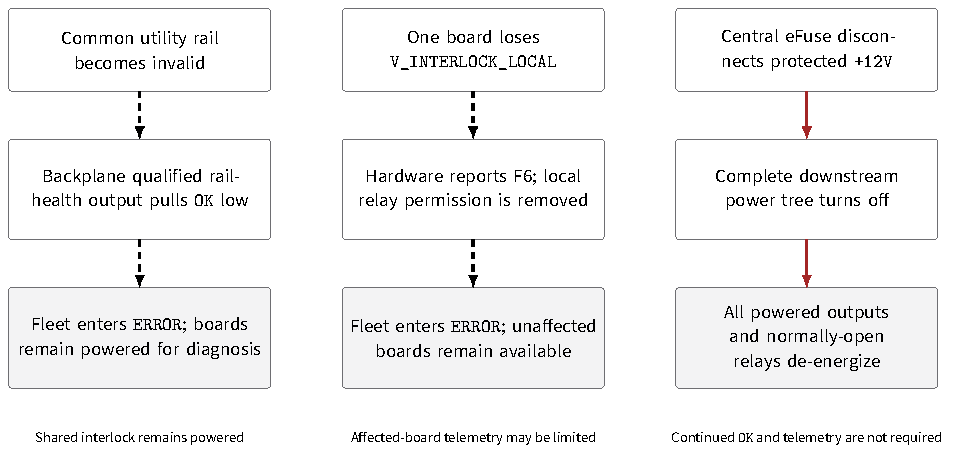
\includegraphics[width=\textwidth]{figures/generated/power_fault_comparison.tikz.pdf}
  \caption{Comparison of a common utility-rail fault, isolated loss of one board's local interlock power, and complete central eFuse cutoff.}
  \label{fig:power-fault-comparison}
\end{figure}

\subsection{A common utility rail becomes invalid}

The controller is powered, possibly armed, when one backplane utility rail leaves its valid range. Its qualified rail-health output pulls \texttt{OK} low directly. The hardware permissive opens detector protection relays, and active boards enter \texttt{ERROR}.

Protected \texttt{+12V} remains present, so boards normally continue to communicate. Main measures the common rails, and the host combines those measurements with board diagnostics. The common recovery process applies even if the voltage returns by itself.

\subsection{One board loses local interlock power}

Assume the shared power system remains valid, but one board loses \texttt{V\_INTERLOCK\_LOCAL} because of a connector branch or local regulator failure, or because an optional board input eFuse disconnects the branch supplying interlock power. The board causes a shared trip either through a direct hardware contribution to \texttt{OK} or through qualified active forwarding that makes main's loop return LOW. Its normally-open detector protection relay also releases as local interlock power collapses. Downstream boards using incoming-loop validity as a hardware permissive can remove local permission before main asserts the shared trip.

The rest of the controller remains powered and enters \texttt{ERROR}. Diagnostics from the affected board may be limited if more of its local power is also lost. Other boards and main still provide evidence. If the board became physically disconnected, the continuity loop may report that condition as an additional cause.

\subsection{The central eFuse removes complete system power}

An unsafe \texttt{+12V\_IN} condition, excessive total current, or protected \texttt{+12V} outside its verified range causes the central eFuse to disconnect protected \texttt{+12V}. Utility converters and all active boards turn off. Normally-open relays de-energize directly.

The shared \texttt{OK} bus and network telemetry do not need to survive this complete cutoff. Safety comes from removing the energy that powered the outputs. Diagnosis then uses the eFuse indication, external supply evidence, and inspection after power is restored. A normal interlock trip does not command this cutoff; it is a separate input-protection action.

\section{Digital Power Collapse Versus Frozen Logic}

Two failures can make a board stop responding while leaving different hardware evidence.

If the processor or FPGA rail collapses, or the FPGA is held in reset, its normal logic cannot be trusted to assert a fault. The fail-safe circuit uses \texttt{V\_INTERLOCK\_LOCAL} and treats loss of the active health signal as unsafe. It pulls \texttt{OK} low without waiting for the watchdog.

If the logic remains powered but freezes, a stale health output might remain in its previous state. The independent hardware watchdog detects the missing pet transitions and pulls \texttt{OK} low. Its output path does not depend on the frozen logic.

In both cases, the fleet enters the same safe response. The difference is diagnostic. A board that still communicates may report watchdog activation or another retained event. A completely unresponsive board is reported as unreachable; investigation considers power, logic, and communication failure without assigning a cause from silence alone. Safe action is not delayed while the host makes that distinction.

\section{Distributed Sequencer-Clock Loss}

Assume the controller is acquiring data when a 100~MHz \texttt{CLOCK} path becomes invalid. The cause could be the source, main-board fanout, bridge path, connector, receiver, or local timing logic.

An affected board observes clock activity using its independent local management or safety clock. It records clock-loss evidence and uses its local trip path to pull \texttt{OK} low. Every function board loses hardware permission and enters the safe error state.

The retained clock-loss record directs investigation to the clock source and distribution. Watchdog timeout is a separate fault associated with processor/control-logic execution and its refresh path.

Figure~\ref{fig:clock-loss-sequence} shows the order. Exact detection and watchdog delays are intentionally not shown.

\begin{figure}[htbp]
  \centering
  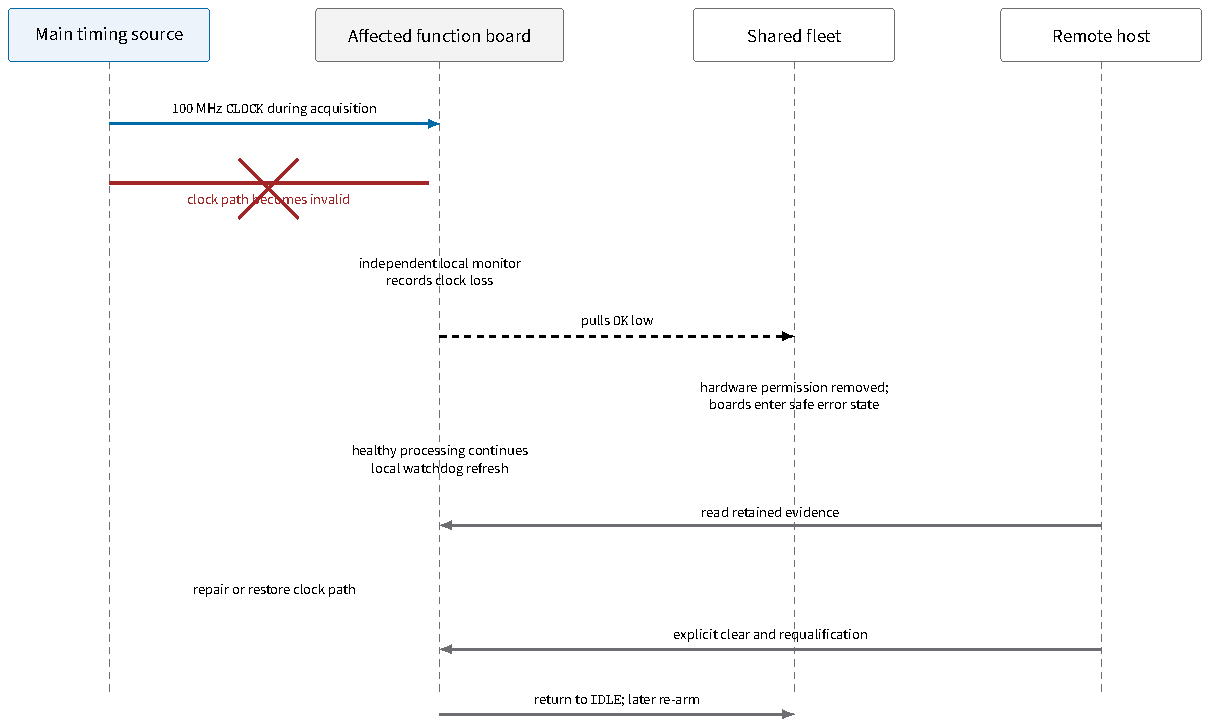
\includegraphics[width=\textwidth]{figures/generated/clock_loss_sequence.tikz.pdf}
  \caption{Clock-loss response, diagnosis, and recovery. Restoring timing does not restart acquisition automatically.}
  \label{fig:clock-loss-sequence}
\end{figure}

The host reads evidence from responding boards to determine whether all paths lost timing or only one branch did. After repair, the common recovery process includes timing requalification.

\section{Host Communication Loss During Acquisition}

Assume the controller is armed and acquiring data when host communication is interrupted. The interruption may affect one board, one switch path, or the complete instrument network; the host application itself may also have frozen. Continued armed operation with an unavailable or unresponsive host is not assumed safe, so boards need not distinguish these causes before taking the protective response.

Every active board maintains its own armed supervision interval. A qualifying operation must demonstrate communication in both directions. A host telemetry request and board response may qualify, providing health visibility during acquisition without a separate heartbeat message. A video board continuing to transmit frames has not, by that fact alone, proved that the host is still reachable.

When the first affected board fails to complete its required interaction within the allowed interval, it records the supervisory event and pulls \texttt{OK} low through its normal local trip path. Hardware relay permission is removed across the fleet, and boards enter \texttt{ERROR}.

After communication returns, the host gathers evidence and follows the common recovery process at the end of this chapter.

\section{Data Overrun Without Supervision Timeout}

Now assume the host and board still complete their qualifying bidirectional interactions, but the network or host cannot absorb all science data. A video buffer overruns or a frame becomes incomplete.

The board reports a data-quality event and identifies the affected acquisition as defined by its ICD. It does not pull \texttt{OK} low solely because science data was lost. Detector safety and data completeness are different concerns.

The acquisition transport follows its defined overrun behavior. It may stop, discard, mark, or recover data according to the instrument design. If valid host interaction continues, the armed supervision timer remains satisfied.

If congestion also prevents the qualifying interaction from completing before its deadline, the independent host-supervision rule applies and the board trips the system. Maximum-load testing must show that this safety interaction cannot be starved indefinitely by science traffic.

\section{Physical Discontinuity}

Assume a board, passive terminator, bridge cable, or connector opens the continuity path. The missing or unpowered item cannot be relied upon to report its own removal.

The continuity path is interrupted, so \texttt{LOOP\_IN} at main becomes invalid. Deterministic main-board logic retains evidence and asserts its contribution to \texttt{OK}. Downstream function boards that use incoming-loop validity as a hardware permissive can remove local detector-facing permission before main asserts \texttt{OK}. The shared \texttt{OK} trip then places the entire powered fleet in the safe error state, including boards upstream of the interruption. This safe-state response does not itself force loop outputs LOW.

If a bridge board loses interlock power, qualified active forwarding makes the loop return LOW; a bridge with passive copper instead reports through a separate hardware contribution to \texttt{OK}. A LOW loop return alone does not distinguish physical disconnection from power loss in an active forwarder. If the cable is physically severed, the loop detects the open path. Both pieces of evidence may appear when one event causes several failures.

An active forwarder may also make its output LOW to report a detected condition that prevents local safety hardware from performing its role. Downstream boards propagate LOW, and main initiates the shared trip. This is an additional reporting path, not a claim that every internal device failure is detected or that the affected board can be located from the return alone. Forwarding resumes when the local condition clears and power/configuration are valid, without waiting for shared-trip recovery; detector outputs still require the normal recovery and arming process.

Removing or inserting boards is therefore not a normal live operation. Service is performed while powered down or already latched safe. The damaged-\texttt{OK}-driver maintenance check described in Chapter~\ref{chap:safety} covers a different latent electronic failure.

\section{Common Scenario Summary}

Table~\ref{tab:scenario-summary} collects the main distinction between the scenarios. It shows the first architectural response, not every later diagnostic possibility.

\begin{table}[htbp]
\centering
\small
\begin{tabularx}{\textwidth}{@{}>{\bfseries\raggedright\arraybackslash}p{0.25\textwidth}>{\raggedright\arraybackslash}p{0.30\textwidth}>{\raggedright\arraybackslash}X@{}}
\toprule
Scenario & First detection or decision & Architectural result \\
\midrule
Board Not Ready at arm & Function-board local arm acceptance & Unsafe arm is rejected; local trip places fleet in \texttt{ERROR} \\
Common utility-rail fault & Backplane qualified rail health & \texttt{OK} low; fleet safe while protected bulk power normally remains \\
One local interlock supply lost & Hardware power-loss reporting and relay disable & \texttt{OK} low directly or through main; local relay releases; fleet safe \\
Complete eFuse cutoff & Central input protection & Complete power tree and normally-open relays de-energize \\
Processor/FPGA power or reset collapse & Interlock-powered fail-safe path & \texttt{OK} low without relying on the failed logic \\
Powered logic freeze & Independent hardware watchdog & \texttt{OK} low after missing valid pet activity \\
Distributed clock loss & Independent-clock activity monitor & \texttt{OK} low; clock and watchdog evidence remain separate \\
Armed host timeout & Board-local supervision timer & Board uses its normal local trip path \\
Data overrun only & Acquisition buffering and transport logic & Data-quality report; no trip solely for the overrun \\
Physical discontinuity & Continuity loop and main-board conversion & Main pulls \texttt{OK} low \\
\bottomrule
\end{tabularx}
\caption{Representative scenarios and their first architectural response.}
\label{tab:scenario-summary}
\end{table}

\section{Generic Fault Correction and Recovery}

Every recoverable fault scenario returns through the same high-level process.

First, hardware has already removed detector-facing permission and the controller is held in \texttt{ERROR.run}. The host reads the evidence that remains available. The operator or control system corrects the external or local condition. Correction may mean restoring a clock, repairing a cable, replacing a board, fixing power, or restoring network service.

Condition correction does not release retained trips by itself. The host requests clear. Each affected board enters \texttt{ERROR.clear}, checks the live condition, and releases its own trip only if allowed. A remaining fault returns that board to \texttt{ERROR.run}.

When clearing succeeds, the controller returns through \texttt{START.wait}. Shared health, timing, monitoring, communication, and applicable board readiness are qualified again. The system then returns to safe \texttt{IDLE}.

Any operational settings or sequencer content invalidated by the event are loaded again. The host verifies the instrument inventory and that board configuration and readiness match the intended operation. A new arm request is required before detector-facing outputs can be enabled.

This common recovery path is deliberate. It avoids special automatic-restart rules for different faults and ensures that restoration is followed by a complete check of the conditions needed for safe operation.

\medskip
\noindent\textit{Chapter sources:} The scenarios combine ADR-001 through ADR-006. ADR-001 controls fault detection, ADR-003 controls state response and recovery, ADR-004 controls timing-loss behavior, ADR-005 controls the power cases, ADR-002 controls readiness and host interaction, and ADR-006 controls data overrun and acquisition traffic.
